\documentclass[11pt]{article}
 
\usepackage[utf8]{inputenc}
\usepackage[latin1]{inputenc}
\usepackage[T1]{fontenc}
\usepackage{lmodern}
\usepackage{eurosym}
\usepackage[french]{babel}
\usepackage{graphicx}

%%% PAGE DIMENSIONS
\usepackage{geometry} % to change the page dimensions
\geometry{a4paper} % or letterpaper (US) or a5paper or....
% \geometry{margin=2in} % for example, change the margins to 2 inches all round
% \geometry{landscape} % set up the page for landscape
%   read geometry.pdf for detailed page layout information

%\usepackage{graphicx} % support the \includegraphics command and options

% \usepackage[parfill]{parskip} % Activate to begin paragraphs with an empty line rather than an indent

%%% PACKAGES
\usepackage{booktabs} % for much better looking tables
\usepackage{array} % for better arrays (eg matrices) in maths
\usepackage{paralist} % very flexible & customisable lists (eg. enumerate/itemize, etc.)
\usepackage{verbatim} % adds environment for commenting out blocks of text & for better verbatim
\usepackage{subfig} % make it possible to include more than one captioned figure/table in a single float
% These packages are all incorporated in the memoir class to one degree or another...


% MATHS
\usepackage{amssymb}


%%COMMANDES
\newcommand{\keyword}[1]{\textsc{#1} }


%%% HEADERS & FOOTERS
\usepackage{fancyhdr} % This should be set AFTER setting up the page geometry
\pagestyle{fancy} % options: empty , plain , fancy
\renewcommand{\headrulewidth}{1pt} % customise the layout...
\renewcommand{\footrulewidth}{1pt}
\lhead{ASD - Labo 3}\chead{}\rhead{N.Mégevand L.Chauffoureaux M. Lemdjo}
\lfoot{}\cfoot{\thepage}\rfoot{}


\title{\vspace{-8mm}\textsc{\huge Algorithmes et structures de données}\\ 
%\vspace{-4 em}
 \large{ Laboratoire 3\\}
\vspace{-1 em}
}
\author{Nathalie Mégevand, Lara Chauffoureaux, Marie Lemdjo} 
\vspace{-1em}

%%%%%%%%%%%%%%%%%%%%%%%%%%%%%%%%%%%%%%%%%%%%%%%%%%%%%%%%%%
\begin{document}

\maketitle
\thispagestyle{fancy}

%\section*{Introduction}
\section*{Estimations théoriques}

\subsection*{Tri par sélection}
Pour le tri par sélection, nous avons une première affectation de iMin dans la boucle extérieur (qui va donc s'exécuter N fois). Puis, probablement une permutation des valeurs de i et iMin.
La boucle interne parcours le tableau de N à i. Cela revient à faire $ \sum^{N}_{k = 0}{(N-k)} = \frac{N(N+1)}{2} $, donc, les instructions à l'intérieur (une comparaison et éventuellement une affectation) s'exécutent $ \frac{N\up{2} + N}{2} $ fois. Nous avons donc au pire : $ N + N + 2*\frac{N\up{2} + N}{2} = N\up{2} + 3N $ opérations.

\subsection*{Tri rapide}

Le tri rapide est un algorithme particulier. Son temps d'exécution en moyenne est de $\mathcal{O}(Nlog(N))$ et de $\mathcal{O}(N^2)$ dans le pire des cas(situation d'un tableau trié de façon  inverse). Il n'utilise pas de tableau annexe pour trier, donc il nécessite très peu de place mémoire pour s'exécuter. Néanmoins, c'est un tri instable. De manière plus détaillée, on a Nlog(N) comparaisons, Nlog(N) permutations, 2N appels de la fonction elle-même et N partitionements. Ce qui nous donne un total de $ Nlog(N) + Nlog(N) + 2N + N = 2Nlog(N) + 3N$ opérations.


\subsection*{Tri par comptage}

Pour le tri par comptage, nous exécutons une première boucle for parcourant tout le tableau à trier afin de trouver le min et le max, dans laquelle nous executons au plus une seule instruction d'affectation et une instruction de comparaison par itération. Puis, nous exécutons une deuxième boucle for parcourant tout le tableau lors de notre phase de comptage. À chaque itération, nous exécutons une incrémentation. Enfin, nous allons replacer chaque élément dans le tableau final, cela revient à parcourir une troisième fois le tableau dans son ensemble, tout en exécutant une instruction par itération. Nous avons donc $2N + N + N = 4N$ instructions pour l'ensemble du tri comptage.


\section*{Résultats empiriques}

\begin{tabular}{|l l l l|}
  \hline
  \multicolumn{4}{|c|}{\textbf{Estimations théoriques}}\footnotemark \\
  \hline
  \textbf{Taille} & \textbf{Tri par sélection} & \textbf{Tri rapide}&  \textbf{Tri par comptage} \\
  \hline
10\up{1}& 1300          & 500     & 400       \\
10\up{2}& 103000        & 7000    & 4000      \\
10\up{3}& 1.003e+07     & 30000   & 40000     \\
10\up{4}& 1.0003e+09    & 1.1e+06 & 40000     \\
10\up{5}& 1.00003e+11   & 1.3e+07 & 400000    \\
10\up{6}& 1.000003e+13  & 1.5e+07 & 4.00e+06  \\
10\up{7}& 1.0000003e+15 & 1.7e+08 & 4.00e+e07 \\
\hline
\end{tabular}

\medskip

\begin{tabular}{|l l l l|}
\hline
\multicolumn{4}{|c|}{\textbf{Résultats empiriques}} \\
\hline
\textbf{Taille} & \textbf{Tri par sélection} & \textbf{Tri rapide}&  \textbf{Tri par comptage} \\
\hline
10\up{1} & 515.2       & 1151.87     & 1424.7  \\
10\up{2} & 26211.9     & 11587.5     & 4874.43  \\
10\up{3} & 1.05628e+06 & 87814.7     & 9936.43  \\
10\up{4} & 5.538e+07   & 530346      & 44343.7  \\
10\up{5} & 5.54646e+09 & 5.36855e+06 & 402290  \\
10\up{6} & 5.9372e+11  & 5.53667e+07 & 4.15027e+06  \\
10\up{7} & NA          & 5.8798e+08  & 4.35604e+07  \\
\hline
\end{tabular}

\footnotetext{Ces temps théoriques on été calculés en prenant arbitrairement 10 nanosecondes de temps d'exécution pour une instruction.}
\medskip

\noindent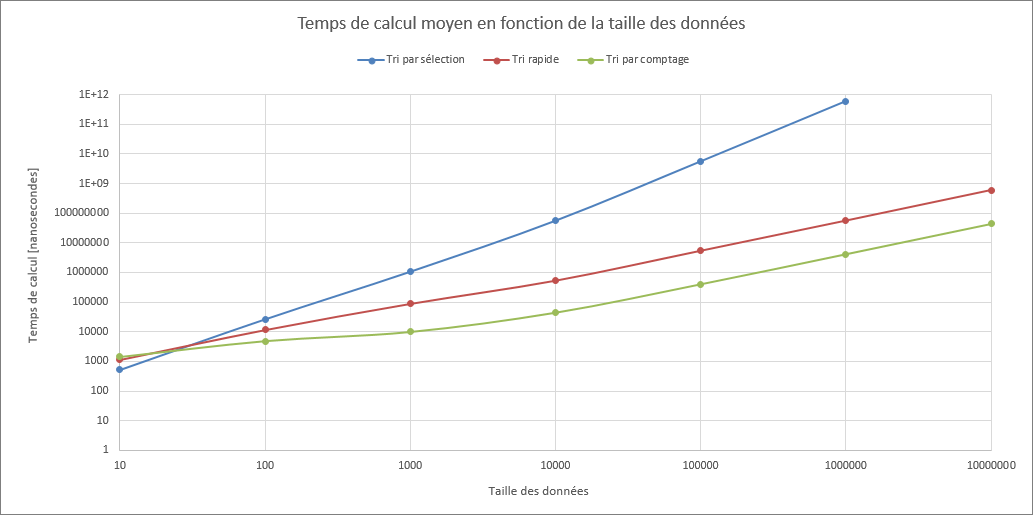
\includegraphics[width=400px]{tests/graphique}

\medskip
\clearpage

\section*{Discussion des résultats}
Après avoir lancé les simulations jusqu'à 10\up{6}, nous avons extrapolé nos résultats et obtenu un résultat théorique de 15h de simulation pour le tri par sélection sur un tableau de 10\up{7} données. Lancer les 30 simulations nous aurait pris $\sim $ 3 semaines. Nous avons donc exécuté les dernières simulations pour les tris rapide et par comptage seulement.

Le graphique ci-dessus (échelle logarithmique sur les deux axes), rend bien visible la différence de performance entre les algorithmes de tris. Le tri par sélection, bien que plus rapide sur des petites tailles de données, devient vite inutilisable pour de plus grands N.

Le tri par comptage quant à lui est très efficace du moment que la taille des tableaux à trier n'est pas trop grande. En effet, ce tri est très rapide, mais demande une grande quantité de mémoire. De plus, ce tri n'est possible que sur des valeurs discrètes.

Le tri rapide est un bon compromis temps-mémoire et peut être utilisé sur toutes les données pouvant être comparées. Il est normal que cet algorithme soit le premier choix pour l'implémentation d'un tri générique. 



%\section*{Conclusion}


\end{document}
